\chapter{General Context and Preliminary Study}

\section*{Introduction}
\addcontentsline{toc}{section}{Introduction}

This chapter presents the context of the Football OS project, the problem
addressed, the study of existing solutions, and the needs that motivate the
proposed solution.

This chapter defines the internship framework and the operational context of
the project. It presents the host company, analyzes the existing environment,
describes the adopted development methodology, and introduces the proposed
solution.

% -------------------------------------------------------
\section{Host Organization Presentation}

\begin{figure}[ht]
    \centering
    
\includegraphics[width=0.35\textwidth]{images/icons/logoPerfAnalysis.png}
    \caption{Perf-Analysis Consulting logo}
    \label{fig:company_logo}
\end{figure}

Perf-Analysis Consulting develops digital tools for professional football
organizations. The internship was conducted within the software engineering
activity of the company and focused on \textbf{Football OS}, with emphasis on
backend foundation services, governance mechanisms, and the Workspace module.

% -------------------------------------------------------
\section{Study of Existing Solutions}

\subsection{Previous Internal Tool}

Before the development of Football OS, the company relied on a previous
internal tool to support part of its operational activities. This solution
helped centralize some document-related work and provided a basic foundation
for internal organization. However, its functional scope remained limited and
its architecture did not fully support the level of modularity, integration,
governance, and scalability required by the target platform.

The previous internal tool is therefore the main existing solution studied in
this report. Its analysis is important because the limitations observed in this
solution directly motivated the design of Football OS as a modular,
governance-oriented, service-based platform.

\begin{table}[ht]
\centering
\caption{Previous internal tool and identified limitations}
\label{tab:previous-internal-tool}
\begingroup
\small
\setlength{\tabcolsep}{4pt}
\renewcommand{\arraystretch}{1.15}
\begin{tabularx}{\textwidth}{|L{3.2cm}|Y|Y|}
\hline
\textbf{Existing Solution} & \textbf{Main Role} & \textbf{Main Limitations} \\
\hline
Previous internal tool & Supported part of the company's operational workflow & Limited modularity, weak centralized governance, limited integrations, insufficient event-driven support, fragmented workspace features, scalability and maintainability limits \\
\hline
\end{tabularx}
\endgroup
\end{table}

\subsection{Limitations of the Previous Internal Tool}

The previous internal tool presented several limitations that reduced its
ability to support the company's evolving operational needs.

\begin{itemize}
    \item \textbf{Limited modularity.} The previous tool was not designed as a
    modular platform. It did not clearly separate gateway, governance,
    workspace, and shared SDK responsibilities, which made evolution and
    maintenance more difficult.

    \item \textbf{Weak governance and authorization model.} Authorization was
    not centralized enough to provide a strong policy-driven governance layer.
    Role-based access and action-level permissions were therefore harder to
    manage consistently across operational workflows.

    \item \textbf{Limited integration with external services.} The tool did
    not provide strong integration with infrastructure such as Keycloak, OPA,
    Kafka, MinIO, and OnlyOffice. This limited its ability to support
    authentication, policy evaluation, event-driven workflows, document
    storage, and online document editing.

    \item \textbf{Insufficient event-driven architecture.} The previous tool
    did not fully support asynchronous signals, audit events, and notification
    projection. This reduced traceability and limited real-time coordination
    between operational activities.

    \item \textbf{Limited document and workspace workflows.} Document
    management, event management, player profiles, notifications, and search
    were not unified within a complete workspace experience. As a result, the
    user experience remained fragmented.

    \item \textbf{Scalability and maintainability limits.} The previous
    solution was harder to extend as business needs evolved. Adding new
    features risked increasing coupling and complexity because the
    architecture did not provide sufficiently explicit service boundaries.

    \item \textbf{Lack of reusable technical foundation.} The solution did not
    include a strong shared SDK layer to standardize contracts, policy checks,
    storage abstraction, canonical lookups, security context, and test
    utilities. This increased duplication and reduced consistency between
    modules.
\end{itemize}

\subsection{Synthesis}

These limitations motivated the design of Football OS as a more modular and
governance-oriented architecture. Football OS addresses the identified issues
by separating responsibilities across dedicated components: the Gateway
provides a secure and standardized entry point, the Governance Service manages
identity, canonical data, policy evaluation, signals, and audit, the Workspace
Service supports documents, calendar events, player profiles, notifications,
search, and OnlyOffice integration, and the Shared SDK provides reusable
contracts and integration mechanisms across backend modules.

% -------------------------------------------------------
\section{Work Methodology}

The project followed an iterative incremental approach. Each iteration produced
an integrated deliverable, then refined technical consistency before extending
scope. This cadence made it possible to build foundational services first and
add operational features progressively. The Shared SDK was developed as a
dedicated standalone foundation iteration before service feature iterations.

\begin{table}[H]
\centering
\caption{Iterative delivery plan used during development}
\label{tab:iteration-plan}
\small
\setlength{\tabcolsep}{4pt}
\renewcommand{\arraystretch}{1.10}
\begin{tabularx}{\textwidth}{|L{2.1cm}|L{3.8cm}|Y|}
\hline
\textbf{Iteration} & \textbf{Objective} & \textbf{Main Deliverables} \\
\hline
\makecell[l]{Iteration\\0} & Shared SDK foundation & Standalone SDK module, shared contracts, security/context helpers, and reusable integration clients consumed by backend services. \\
\hline
Iteration 1 & Platform foundation & API Gateway routing baseline, service structure, and Docker-based environment. \\
\hline
Iteration 2 & Governance & Actors, roles, players, policy integration, and audit mechanisms. \\
\hline
Iteration 3 & Workspace documents & Document upload, metadata handling, storage integration, and OnlyOffice connection. \\
\hline
Iteration 4 & Calendar and events & Event management, attendees, tasks, and notification workflows. \\
\hline
Iteration 5 & Integration and validation & Frontend integration, functional validation, and corrective refinements. \\
\hline
\end{tabularx}
\normalsize
\end{table}

The iteration sequence reflects a risk-first strategy: shared contracts and
security foundations were stabilized before feature expansion. This reduced
late-stage rework on cross-cutting concerns such as authorization and
traceability.

The approach still involved a known limitation: front-loading architecture can
delay visible functional outcomes in early milestones. In this project, that
trade-off was accepted because governance consistency was a prerequisite for
reliable document and event workflows.

% -------------------------------------------------------
\section{Proposed Solution and Positioning}

To address the identified gaps, the project proposes \textbf{Football OS} as a
unified workspace for football club operations.

The platform is structured around two complementary layers:
\begin{itemize}
    \item \textbf{Governance layer:} identity context, roles, permissions, canonical players and teams, and audit traceability,
    \item \textbf{Workspace layer:} documents, events, notifications, search, and player profile consultation.
\end{itemize}

This structure is supported by a modular architecture that separates concerns
between Gateway, Governance, Workspace, and Shared SDK modules. The separation
improves maintainability and enables controlled future extension without
restructuring the entire platform.

From an engineering perspective, this design solved the immediate need for
clear ownership boundaries while preserving extensibility for future club
workflows. Its main remaining constraint is integration overhead: each new
feature must align with Gateway routing, Governance policy, and Workspace data
contracts.

% -------------------------------------------------------

\section{Requirements Specification}

This chapter formalizes the needs of Football OS through measurable
requirements, actor definitions, and use-case models. The focus is on expected
system behavior and access rules, independently from implementation details.

% =====================================================
\section{Functional Requirements}

Functional requirements are summarized in
Table~\ref{tab:functional-requirements}, with identifiers, actors, priorities,
and delivery status in the current project scope.

\begin{table}[ht]
\centering
\caption{Functional requirements of Football OS}
\label{tab:functional-requirements}
\begingroup
\small
\setlength{\tabcolsep}{4pt}
\renewcommand{\arraystretch}{1.12}
\begin{tabularx}{\textwidth}{|C{1.3cm}|Y|L{2.6cm}|C{1.4cm}|C{2.3cm}|}
\hline
\textbf{ID} & \textbf{Requirement} & \textbf{Main Actor} & \textbf{Priority} & \textbf{Status} \\
\hline
FR-01 & Authenticate through an external identity provider and enforce protected access. & All platform users & High & Implemented \\
\hline
FR-02 & Manage users and roles for administrative governance. & Club Administrator & High & Partial \\
\hline
FR-03 & Manage canonical club data (players and teams) with controlled updates. & Club Administrator & High & Partial \\
\hline
FR-04 & Upload, consult, and archive documents under authorization rules. & Authorized staff & High & Implemented \\
\hline
FR-05 & Support document versioning and online viewing or editing. & Authorized staff & High & Implemented \\
\hline
FR-06 & Manage calendar events, attendees, and task coordination. & Head Coach / Club Administrator & High & Implemented \\
\hline
FR-07 & Consult player profiles with role-based filtering. & Authorized staff & High & Partial \\
\hline
FR-08 & Generate and consult notifications for operational updates. & Authorized staff & Medium & Implemented \\
\hline
FR-09 & Search workspace resources with permission filtering. & Authorized staff & Medium & Implemented \\
\hline
FR-10 & Enforce access control and activity tracking for accountability. & Backend services & High & Implemented \\
\hline
\end{tabularx}
\endgroup
\end{table}

The status distribution in Table~\ref{tab:functional-requirements} reflects an
intentional prioritization: security-critical and workflow-critical functions
were completed first, while some advanced governance and profile capabilities
remain partially implemented.

% =====================================================
\section{Non-functional Requirements}

Non-functional requirements are formalized in
Table~\ref{tab:non-functional-requirements} to clarify quality expectations and
their validation approach.

\begin{table}[ht]
\centering
\caption{Non-functional requirements of Football OS}
\label{tab:non-functional-requirements}
\begingroup
\small
\setlength{\tabcolsep}{4pt}
\renewcommand{\arraystretch}{1.12}
\begin{tabularx}{\textwidth}{|C{1.4cm}|L{2.4cm}|Y|Y|}
\hline
\textbf{ID} & \textbf{Quality Attribute} & \textbf{Requirement} & \textbf{Validation Method} \\
\hline
NFR-01 & Security & Enforce authenticated access, role-based authorization, and protected sensitive exchanges. & Security tests, policy checks, and access-control cases. \\
\hline
NFR-02 & Usability & Provide clear daily workflows with understandable user feedback. & UI scenario reviews and user acceptance checks. \\
\hline
NFR-03 & Performance & Keep response times acceptable for common operations such as documents, events, and search. & Workflow-oriented performance checks. \\
\hline
NFR-04 & Maintainability & Preserve modular separation of concerns and reusable cross-service contracts. & Architecture review and module inspections. \\
\hline
NFR-05 & Reliability & Maintain consistent behavior and controlled failure handling in normal operations. & Integration and error-handling validation. \\
\hline
NFR-06 & Traceability & Record significant operations for audit and accountability. & Audit-log verification and end-to-end trace checks. \\
\hline
\end{tabularx}
\endgroup
\end{table}

\subsection{Prioritization Rationale and Trade-offs}

The requirement baseline follows a sequencing logic aligned with project risk.
Security, traceability, and maintainability were treated as structural
qualities because they condition the reliability of all business features.
Usability and performance were addressed progressively once secure routing and
policy enforcement were stable.

This prioritization introduced a predictable trade-off. Focusing early effort
on architecture and governance reduced late integration risk, but it delayed
the full maturity of some user-facing capabilities such as profile depth and
advanced search behavior. The resulting scope remains coherent for a PFE
prototype and provides a controlled base for incremental evolution.

% =====================================================
\section{Use Case Modeling}

The use-case and actor models in this chapter follow UML notation conventions
for behavioral modeling and diagram semantics \cite{uml-spec}.

\subsection{Actor Model}

Actors are consolidated in Table~\ref{tab:actor-model}.

\begin{table}[H]
\centering
\caption{Actor model of Football OS}
\label{tab:actor-model}
\small
\setlength{\tabcolsep}{4pt}
\renewcommand{\arraystretch}{1.10}
\begin{tabularx}{\textwidth}{|L{3.0cm}|C{1.9cm}|Y|}
\hline
\textbf{Actor} & \textbf{Type} & \textbf{Role in the system} \\
\hline
Club Administrator & Human & Manages users, roles, governance data, and high-level operational permissions. \\
\hline
Head Coach & Human & Manages events and operational coordination for football activities. \\
\hline
Coaching Staff & Human & Consults events, documents, and player-related operational information. \\
\hline
Medical Staff & Human & Accesses authorized medical and player-related information. \\
\hline
Identity Provider & Technical & Authenticates users and provides identity/session context. \\
\hline
Document Editor & Technical & Supports online document viewing and editing workflows. \\
\hline
Object Storage Provider & Technical & Stores document binary content and file versions. \\
\hline
Governance Policy Service & Technical & Evaluates authorization decisions for protected actions. \\
\hline
Canonical Player Data Provider & Technical & Provides canonical player identity references used by workspace features. \\
\hline
\end{tabularx}
\normalsize
\end{table}

\subsection{Global Use Case Diagram}

The global platform use-case diagram provides a high-level view of the
interactions between Football OS and its actors. Figure~\ref{fig:global-usecase}
presents the global use-case view of Football OS. Human actors are represented
as primary users of the platform, while technical actors represent external
systems involved in authentication, policy evaluation, document editing, object
storage, and canonical player data retrieval. The diagram summarizes the main
services offered by the platform without exposing internal implementation
details, since detailed processing flows are presented later in the design
chapter.

\begin{figure}[H]
    \centering
    \captionsetup{skip=4pt}
    \makebox[\textwidth][c]{%
        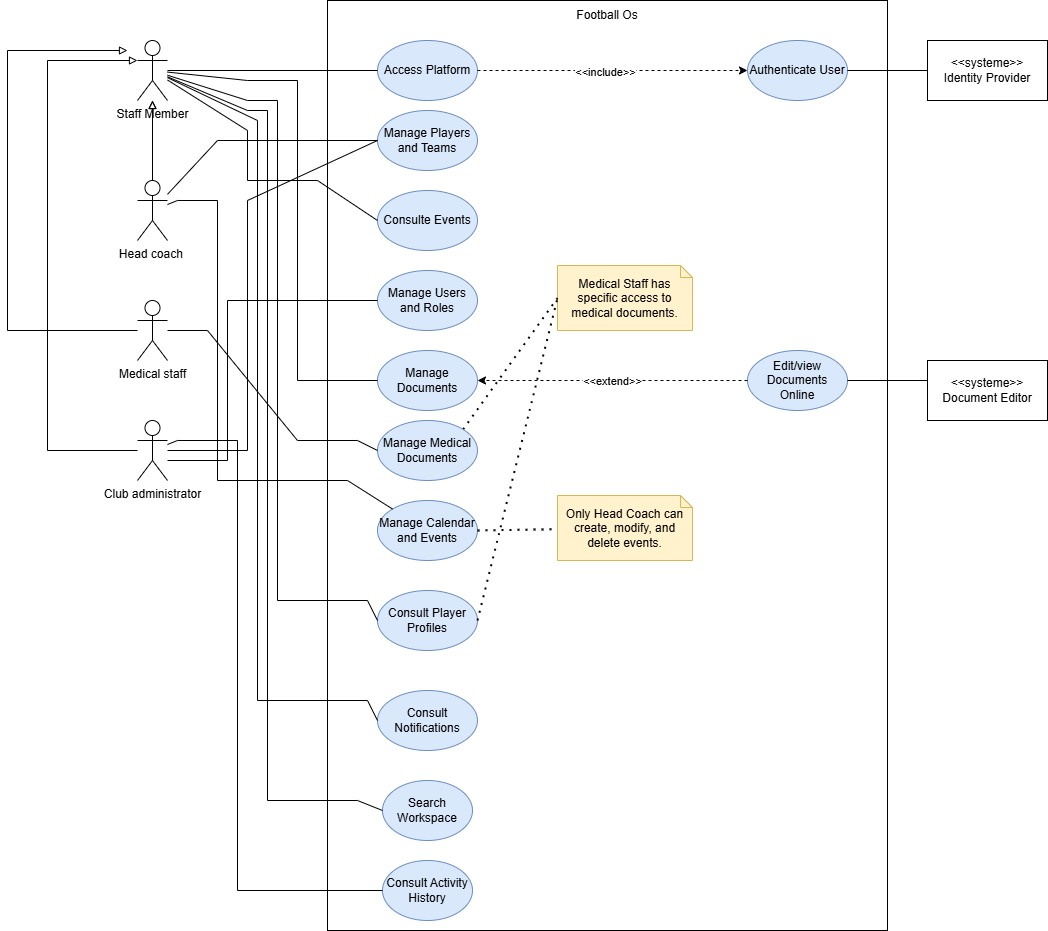
\includegraphics[width=0.90\textwidth]{images/usecase/footballosgeneralusecase.drawio (1).drawio (1).png}%
    }
    \caption{General use case diagram of the Football OS platform}
    \label{fig:global-usecase}
\end{figure}

The use-case descriptions below formalize the principal operational flows in
the current scope. They are written as behavioral contracts so that design and
implementation choices can later be validated against explicit preconditions,
access rules, and postconditions.

%\subsubsection*{Access Football OS Platform}
\small
\begin{table}[H]
\centering
\caption{Use-case description: Access Football OS Platform}
\label{tab:uc-access-platform}
\begin{tabular}{|p{4.0cm}|p{10.0cm}|}
\hline
\textbf{Use Case} & Access Football OS Platform \\
\hline
\textbf{Primary Actor} & Club Administrator / Head Coach / Coaching Staff / Medical Staff \\
\hline
\textbf{Secondary Actor} & Identity Provider \\
\hline
\textbf{Objective} & Authenticate the user and grant access to authorized platform features. \\
\hline
\textbf{Preconditions} & User account exists and identity provider is reachable. \\
\hline
\textbf{Main Scenario} &
\begin{enumerate}
    \item The user opens the platform,
    \item The system redirects authentication to the identity provider,
    \item The user authenticates successfully,
    \item The system resolves role context and grants authorized access.
\end{enumerate}
\\
\hline
\textbf{Alternative / Exception Scenario} & Authentication failure or invalid token; access is denied and the user remains outside protected features. \\
\hline
\textbf{Business Rules / Access Rules} & Protected features require authenticated identity. Visible modules depend on role permissions. \\
\hline
\textbf{Postconditions} & Authenticated session is established with role-scoped access rights. \\
\hline
\end{tabular}
\end{table}
Table~\ref{tab:uc-access-platform} specifies the authentication-oriented
platform-access use case.
\normalsize

\subsection{Calendar and Event Management}

\begin{figure}[H]
\centering
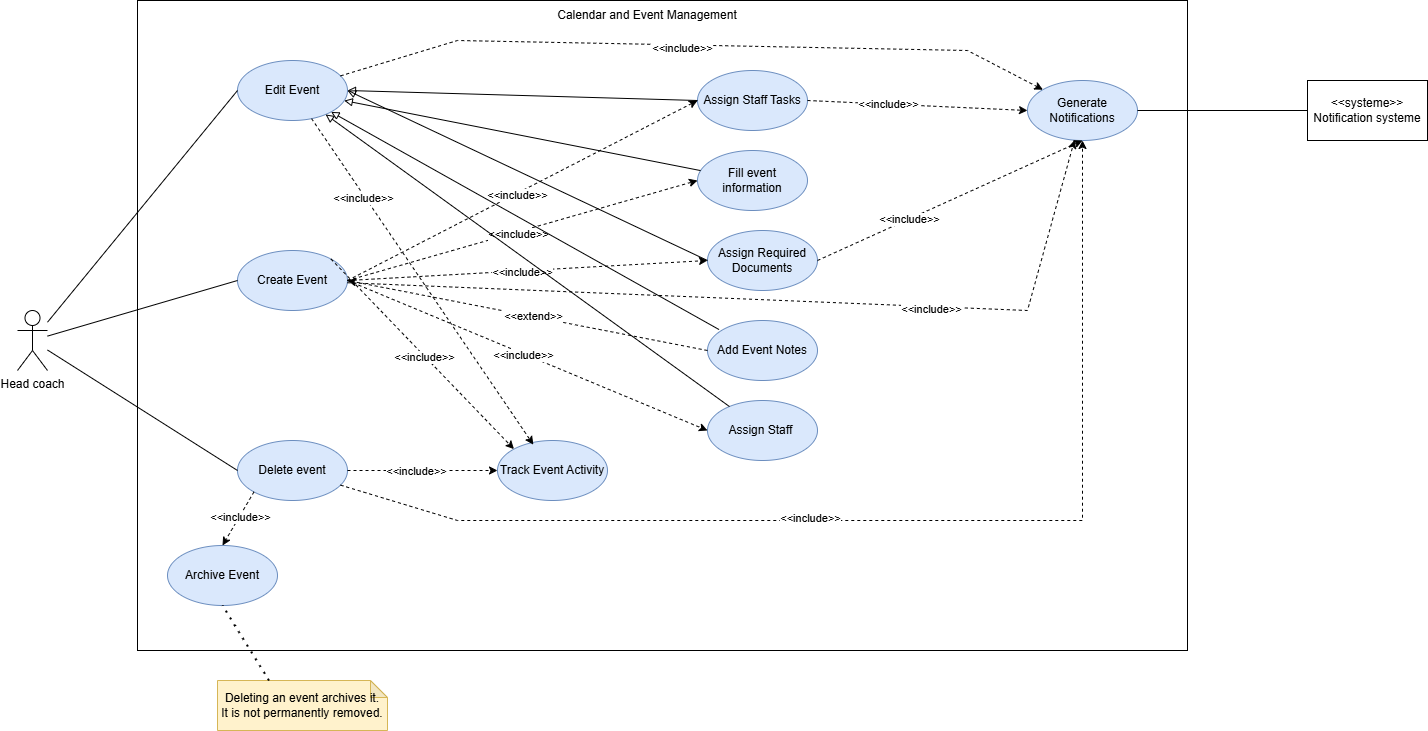
\includegraphics[width=0.92\textwidth, height=0.30\textheight, keepaspectratio]{images/usecase/Calendar and Event Management.png}
\caption{Calendar and event management use case diagram}
\label{fig:calendar-usecase}
\end{figure}

Figure~\ref{fig:calendar-usecase} illustrates the actor interactions for event
planning, consultation, and archive operations.

\small
\renewcommand{\arraystretch}{1.05}
\begin{table}[H]
\centering
\caption{Use-case description: Calendar and Event Management}
\label{tab:uc-calendar-events}
\begin{tabular}{|p{4.0cm}|p{9.8cm}|}
\hline
\textbf{Use Case} & Calendar and Event Management \\
\hline
\textbf{Primary Actor} & Head Coach / Club Administrator (management), authorized staff (consultation) \\
\hline
\textbf{Objective} & Plan, update, consult, and archive operational events and related assignments. \\
\hline
\textbf{Preconditions} & User is authenticated and has calendar access rights. \\
\hline
\textbf{Main Scenario} &
\begin{enumerate}
    \item The user opens the calendar module,
    \item The user creates, updates, consults, or archives an event,
    \item The system validates permissions and persists the operation,
    \item The system updates related attendees, tasks, and notifications when applicable.
\end{enumerate}
\\
\hline
\textbf{Alternative / Exception Scenario} & Unauthorized update request, invalid event data, or unavailable service causes rejection with error feedback. \\
\hline
\textbf{Business Rules / Access Rules} & Event management actions are restricted to authorized roles. Delete behavior is treated as archive action, not hard deletion. \\
\hline
\textbf{Postconditions} & Event state is updated according to the accepted operation and authorized users are notified when required. \\
\hline
\end{tabular}
\end{table}
Table~\ref{tab:uc-calendar-events} formalizes the calendar and event use-case
contract.
\normalsize
\renewcommand{\arraystretch}{1}

\subsection{Document Management}

This subsection defines document-management behavior and integration points
through its use-case contract.

\begin{figure}[H]
\centering

\includegraphics[width=0.92\textwidth, height=0.30\textheight, keepaspectratio]{images/usecase/documentManagment.drawio (1).png}
\caption{Document management use case diagram}
\label{fig:document-management-usecase}
\end{figure}

\noindent Figure~\ref{fig:document-management-usecase} illustrates the main
actor interactions for document upload, consultation, editing, versioning, and
archiving operations.

\small
\renewcommand{\arraystretch}{1.05}
\begin{table}[H]
\centering
\caption{Use-case description: Document Management}
\label{tab:uc-document-management}
\begin{tabular}{|p{4.0cm}|p{9.8cm}|}
\hline
\textbf{Use Case} & Document Management \\
\hline
\textbf{Primary Actor} & Club Administrator / Head Coach / Coaching Staff / Medical Staff \\
\hline
\textbf{Secondary Actors} & Object Storage Provider / Document Editor \\
\hline
\textbf{Objective} & Manage document upload, consultation, versioning, editing, and archiving under controlled access. \\
\hline
\textbf{Preconditions} & User is authenticated and authorized for the requested document action. \\
\hline
\textbf{Main Scenario} &
\begin{enumerate}
    \item The user opens the document module and selects an action,
    \item The system validates permissions and applies business rules,
    \item The system stores or retrieves document metadata and versions,
    \item The system invokes online editor integration when editing is requested.
\end{enumerate}
\\
\hline
\textbf{Alternative / Exception Scenario} & Upload failure, editor unavailability, or unauthorized access attempt triggers a controlled error response. \\
\hline
\textbf{Business Rules / Access Rules} & Document visibility depends on role and category. Medical documents are restricted to medical staff and explicitly authorized roles. \\
\hline
\textbf{Postconditions} & Document state and version history are updated according to authorized operations. \\
\hline
\end{tabular}
\end{table}
Table~\ref{tab:uc-document-management} defines the detailed scenarios and
access constraints of document management.
\normalsize
\renewcommand{\arraystretch}{1}

\subsection{Player Profile Consultation}

Player profile consultation requires policy-driven visibility because sensitive
medical and administrative information must remain restricted by role.

\begin{figure}[H]
\centering
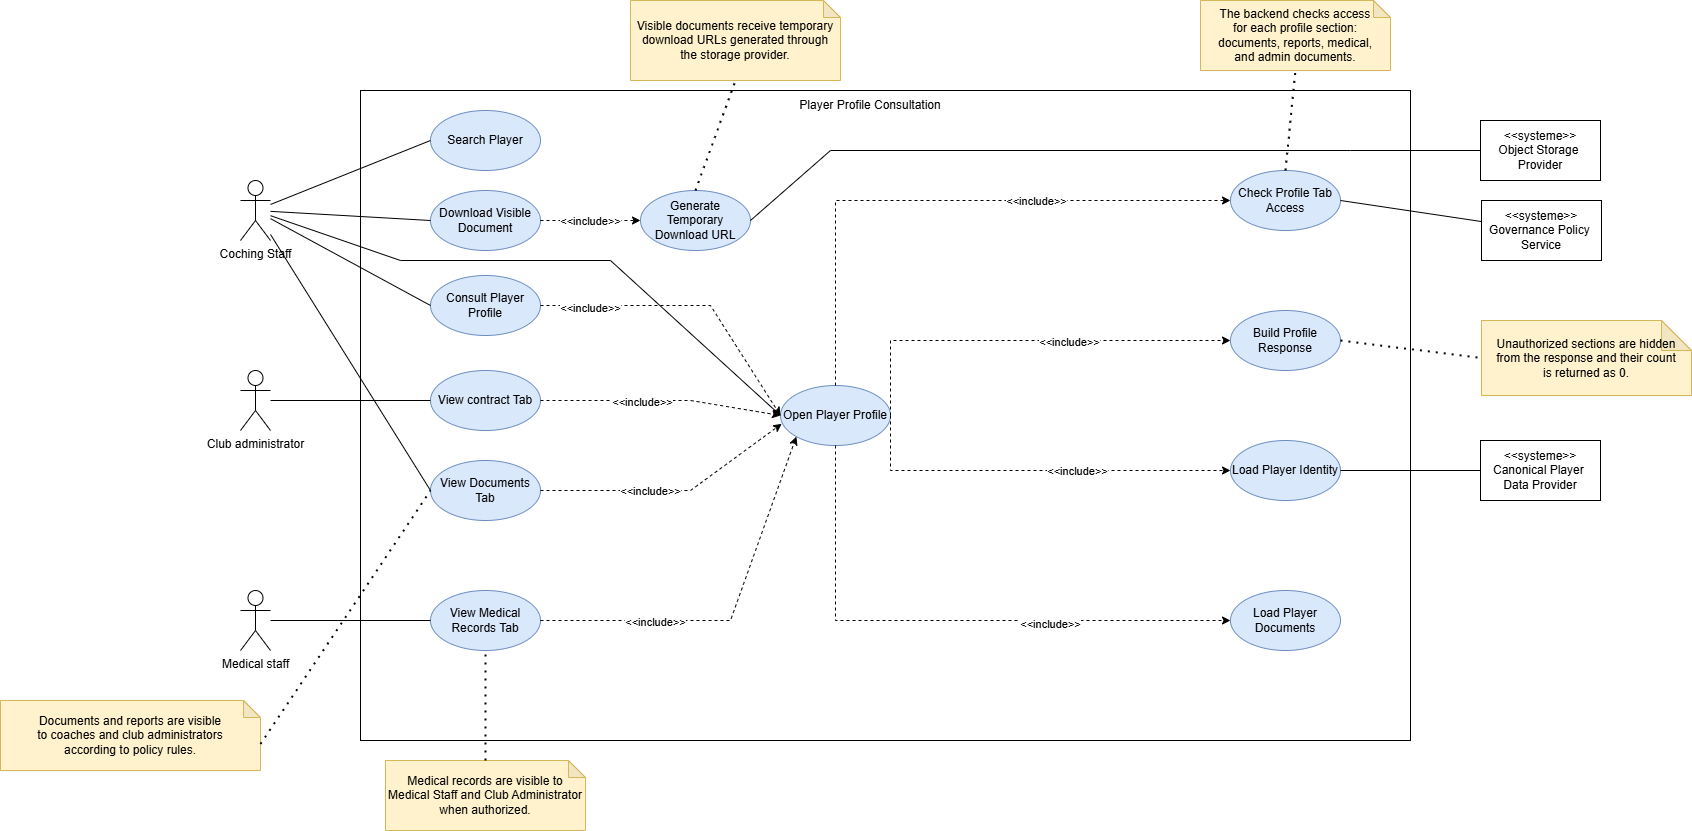
\includegraphics[width=0.92\textwidth, height=0.30\textheight, keepaspectratio]{images/usecase/Player Profile Consultation.drawio (1).png}
\caption{Player profile consultation use case diagram}
\label{fig:player-profile-usecase}
\end{figure}

\small
\renewcommand{\arraystretch}{1.05}
\begin{table}[H]
\centering
\caption{Use-case description: Consult Player Profile}
\label{tab:uc-player-profile}
\begin{tabular}{|p{4.0cm}|p{9.8cm}|}
\hline
\textbf{Use Case} & Consult Player Profile \\
\hline
\textbf{Primary Actor} & Club Administrator / Head Coach / Coaching Staff / Medical Staff \\
\hline
\textbf{Secondary Actors} & Canonical Player Data Provider / Governance Policy Service \\
\hline
\textbf{Objective} & Display player profile sections according to user permissions and available data. \\
\hline
\textbf{Preconditions} & User is authenticated and the selected player exists in reference data. \\
\hline
\textbf{Main Scenario} &
\begin{enumerate}
    \item The user selects a player profile,
    \item The system retrieves canonical and workspace-linked information,
    \item The system evaluates section-level permissions,
    \item The system displays only authorized profile sections.
\end{enumerate}
\\
\hline
\textbf{Alternative / Exception Scenario} & Unknown player, unavailable linked data, or insufficient permission leads to partial display or access rejection. \\
\hline
\textbf{Business Rules / Access Rules} & Sensitive profile content, especially medical information, is visible only to authorized roles. \\
\hline
\textbf{Postconditions} & User receives a role-filtered profile view consistent with policy decisions. \\
\hline
\end{tabular}
\end{table}
Table~\ref{tab:uc-player-profile} specifies the profile-consultation behavior
under role-based restrictions.
\normalsize
\renewcommand{\arraystretch}{1}

\section{Engineering Analysis of the Specification}

Taken together, the requirement tables and use-case contracts show that Football
OS is governed less by isolated CRUD operations than by controlled interactions
between identity, policy, and operational data. This is why the specification
emphasizes access conditions and audit consequences alongside functional goals.

Compared with a purely user-story-oriented specification, the selected approach
is more explicit about authorization boundaries and exception paths, which
improves downstream architectural traceability. Its limitation is higher
documentation density; however, that cost is justified by the security and
accountability constraints of the targeted domain.

\section*{Conclusion}
\addcontentsline{toc}{section}{Conclusion}

This chapter consolidates the internship context, the study of existing
solutions, and the specification of functional and non-functional needs. This
foundation justifies the architecture and design choices presented in the next
chapter.

